% +--------------------------------------------------------------------+
% | Sample Chapter
% |
% | This file provides examples of how to
% | - insert a figure with a caption
% | - construct a table with a caption
% | - create subsections within the chapter
% | - insert a reference to a Figure or Table
% | - make a citation
% +--------------------------------------------------------------------+

\cleardoublepage

% +--------------------------------------------------------------------+
% | Replace "Chapter Title" below with the title of your chapter.  LaTeX
% | will automatically number the chapters.
% +--------------------------------------------------------------------+

\chapter{Introducción}
% \label{ch:chapter1}
\label{makereference}

Tal y como se cuenta en~\citet{DEFANTI1991247}, los científicos computacionales
basan su trabajo en fuentes de datos de gran volumen. Sin embargo, estos datos
tienen tal magnitud que los científicos se ven, a menudo, superados. Entre las
fuentes de datos de gran volumen se encuentran:

\begin{itemize}
		\item Supercomputadores
		\item Inteligencia militar, satélites, datos astronómicos y de tiempo atmosférico
		\item Sondas enviando datos desde otros planetas
		\item Radio telescopios terrestres
		\item Instrumentos capturando temperaturas oceánicas, movimientos tectónicos y 
				actividad volcánica y sísmica
		\item Escáneres médicos empleando distintas técnicas de imagen como tomografía, 
				resonancias magnéticas, etc
\end{itemize}

Simplemente con un formato numérico, el cerebro humano es incapaz de interpretar
gigabytes de datos cada día, resultando en mucha información desperdiciada. De
aquí surge la necesidad de una alternativa a los números. La posibilidad de los
científicos para visualizar cómputos complejos y simulaciones es absolutamente
esencial para asegurar la integridad de análisis y predicciones, así como
presentar esta información al resto.\\

Esta capacidad de visualización se hace especialmente importante en el ser
humano, puesto que, de todas nuestras funciones cerebrales, nuestro sistema de
visión es el que mayor capacidad de procesamiento de información tiene. Según
expertos en conocimiento, el procesamiento de información en humanos tiene dos
formas: preconsciente y consciente. El procesamiento de información
preconsciente es involuntario, similar a la respiración. Este es el tipo de
procesamiento que se da en información gráfica.
~\citet{Rohrer:2000:SBI:510378.510552}

Teniendo esto en cuenta y el hecho de que cada persona tiene una capacidad de
vision espacial diferente, la informática gráfica puede ayudar a aquellos que
tienen una mayor dificultad y que, de otro modo, serían incapaces de visualizar
conceptos complejos.

Estos hechos muestran una necesidad ha resultado en el surgimiento, en la última
década, de una disciplina totalmente independiente, la visualización científica. 

\section{Motivación}
\label{makereference1.1}

La importancia de lo expuesto anteriormente sirve como suficiente motivación,
aunque a esto se ha de añadir el reto personal de, con este trabajo, aprender
y entender un área de la informática que no forma parte del itinerario en mi
formación, como es la informática gráfica, y que engloba muchas de las materias
vistas hasta ahora tanto en ingeniería informática como en matemáticas.\\

Además, esta rama dentro de la investigación científica es relativamente
reciente, asociándose su nacimiento en 1987 al
artículo~\citet{McCormick:1988:VSC:43965.43966}, por lo que aún hay muchos retos
y problemas por resolver, haciendo su estudio muy interesante.

\section{Objetivos}
\label{makereference1.2}

El objetivo principal de este trabajo es el de aprender el funcionamiento básico
de los gráficos y la aplicación de éstos a la investigación científica.
Este objetivo se puede desglosar en otros subobjetivos más concretos y que
marcan la línea de trabajo:
\begin{enumerate}
		\item Comprender el pipeline de gráficos y la utilidad y funcionamiento
				de los shaders, así como aprender el lenguaje GLSL para su
				escritura.
		\item Aprender las técnicas más conocidas de visualización científica y
				cómo desarrollar shaders que las implementen.
		\item Desarrollar una aplicación que ponga de manifiesto lo aprendido,
				desarrollando shaders que ilustren algunas de las técnicas
				vistas.
\end{enumerate}

\section{Plan de trabajo}
\label{makereference1.3}
Con estos objetivos en mente, se desarrolló el siguiente plan de trabajo,
acordado en reuniones iniciales entre tutora y autor del trabajo.

\begin{itemize}
		\item \textbf{Toma de contacto con OpenGL} Durante esta fase se leyeron
				tutoriales sobre OpenGL y se experimentó con diversos shaders y
				librerías para familiarizarse con la tecnología, a la vez que se
				aprendía el lenguaje GLSL.
		\item \textbf{Documentación} Durante la duración completa del proyecto
				se llevó a cabo una documentación acerca de las distintas
				fuentes de información, con el objetivo de no olvidar incluir
				partes importantes en la memoria.
		\item \textbf{Comunicación con el tutor} Se concretaron diversas
				reuniones con la tutora durante las partes intensivas del
				proyecto con el fin de mostrar avances y acordar los siguientes
				pasos. Asimismo, se mantuvo una comunicación mediante correo
				electrónico para aquellas dudas menores que surgieron durante la
				realización del trabajo.
		\item \textbf{Preparación del entorno de desarrollo} Durante esta fase
				se preparó el equipo, instalando las librerías y programas
				necesarios para el correcto funcionamiento de la aplicación.
		\item \textbf{Desarrollo de la aplicación} Una vez preparado el entorno,
				se continuó durante toda la duración del trabajo con el
				desarrollo de la aplicación, incluyendo cada vez nuevas
				capacidades.
		\item \textbf{Redacción de la memoria} Se inició la redacción de la
				memoria una vez se tenían conocimientos suficientes, a mitad de
				la elaboración del trabajo. Una vez comenzada la redacción, se
				fue reeditando y mejorando en un proceso iterativo.
\end{itemize}

\section{Estructura de la memoria}
\label{makereference1.4}

El siguiente capítulo, \textbf{OpenGL y DirectX}~\ref{makereference2}, presenta
las dos grandes especificaciones dentro de la informática gráfica, centrándose
en OpenGL y analizando sus características, capacidades y debilidades, así como
las diferencias entre ambas.\\

Posteriormente, el capítulo \textbf{Shaders y Visualización
Científica}~\ref{makereference3} explora las técnicas más comunes dentro del
campo de visualización científica y qué tipos de shaders son útiles para cada
una de ellas, introduciendo algunos de los que más adelante se presentarán junto
a la aplicación.\\

En el capítulo \textbf{Aplicación}~\ref{makereference4} se presenta la
aplicación desarrollada, explicando el diseño, capacidades, experimentos
realizados\ldots\\

Por último el capítulo \textbf{Conclusiones y Trabajo
Futuro}~\ref{makereference5} incluye un análisis del trabajo realizado, el nivel
de cumplimiento de los objetivos propuestos y posibles líneas de trabajo
futuro.\\

\begin{table}[b]
	% \begin{center}
		\begin{tabular}[b]{|c|}
			\hline
			\\
			El código de la aplicación desarrollada puede encontrarse en el
			siguiente enlace:\\
			http://github.com/davidfdezalcoba/TFG\\
			\\
			\hline
		\end{tabular}
	% \end{center}
\end{table}

% How to insert figures:
% \begin{figure}[htb]%t=top, b=bottom, h=here
% 
% 	\begin{center}
% 	    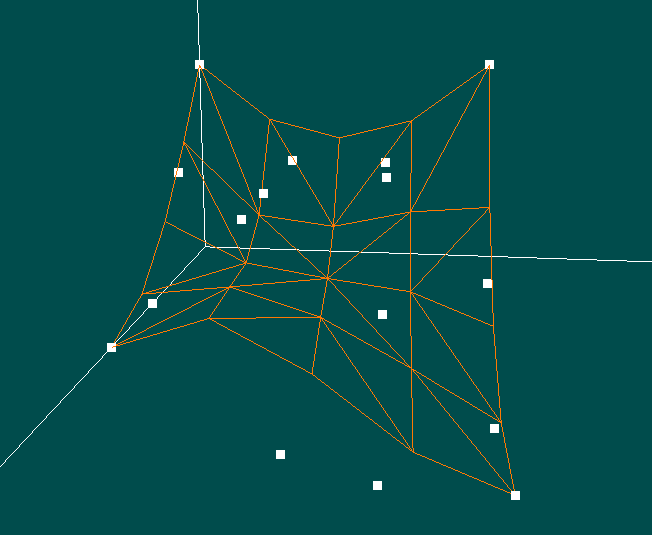
\includegraphics[height=2.5in]{figures/lowressur.png}
% 	    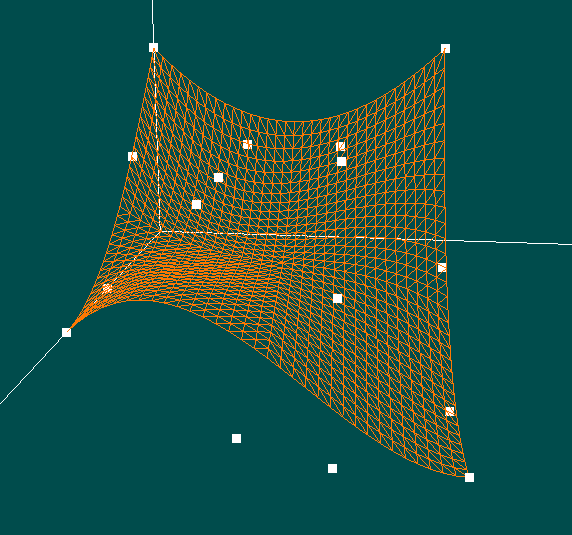
\includegraphics[height=2.5in]{figures/highressur.png}
% 	\end{center}
% 
%     \caption[Optional: Short caption to appear in List of
%     Figures]{Full caption to appear below the Figure}
% 
%     \label{figure1}
% 
% \end{figure}

% +--------------------------------------------------------------------+
% |To create cross-references to figures, tables and segments
% |of text, LaTeX provides the following commands:
% |   \label{marker}
% |   \ref{marker}
% |   \pageref{marker}
% | where {marker} is a unique identifier.
% |
% | In the line above, we use \label{figure1} to mark a location
% | we wish to refer to later.  LATEX replaces \ref by the number of
% | the chapter, section, subsection, figure, or table after which the
% | corresponding \label command was issued. \pageref prints the page
% | number of the page where the \label command occurred.
% |
% +--------------------------------------------------------------------+

% +--------------------------------------------------------------------+
% | The table is created with this command
% |
% | \begin{tabular}[pos]{table spec}
% |
% | The "pos" argument specifies the vertical position of the table relative to
% | the baseline of the surrounding text.  Use t, b, or c to specify alignment
% | at the top, bottom, or center.
% |
% | The "table spec" command defines the format of the table
% |   l for a column of left-aligned text
% |   r for a column of right-aligned text
% |   c for centered text
% |   p{width} for a column containing justified text with line breaks
% |   | for a vertical line
% +--------------------------------------------------------------------+

% +--------------------------------------------------------------------+
% | Replace \section headings below with the title of your
% | subsections.  LaTeX will automatically number the subsections 1.1,
% | 1.2, 1.3, etc.
% +--------------------------------------------------------------------+

% +--------------------------------------------------------------------+
% | Some insight about citations

% | In this paragraph, we want to refer to Fig.~\ref{figure1}
% | mentioned at the beginning of this chapter.  We also refer to the
% | Table~\ref{table1}.
% | 
% | \section{Making a Reference to a Chapter Subsection}
% | \label{makereference1.2}
% | 
% | In this section, we refer back to text mentioned in
% | Section~\ref{makereference1.1} on page~\pageref{makereference1.1}.
% +--------------------------------------------------------------------+
